%//==============================--@--==============================//%
\subsection{2.1 Modulação de Amplitude}
\label{subsec:AM}

\begin{theo}[\underline{Modulação de Amplitude} \cite{Haykin2007}]{def:AM}\label{def:AM}
     ``Amplitude modulation (AM) is formally defined as a process in which the amplitude of the carrier wave is varied about a mean value linearly with the message signal.''
\end{theo}

\subsubsection[2.1.1 Double Sideband AM]{$\rightarrow$ Double Sideband AM}
\label{subsubsec:conditions}
Supondo uma portadora sinusoidal $c(t)$ de fase nula:
$$
    c(t) = A_c\cos{(2\pi f_c t)}
$$
\noindent E uma mensagem (\textit{information-bearing signal, message signal}) $m(t)$, uma onda AM-DSB pode ser representada da seguinte forma:
$$
    \boxed{s(t) = \left[1 + k_am(t)\right]A_c\cos{(2\pi f_c t)}}
$$
\noindent onde $k_a$ denomina-se \textit{amplitude sensitivity} e é dependente do modulador que gera a mensagem modulada $s(t)$.
\\\\
A informação da mensagem reside no envelope da onda modulada, que é definido como a amplitude de $s(t)$, i.e., $[1 + k_a m(t)]$. É expectável que o envelope da onda modulada possua a mesma forma da mensagem, garantindo a satisfação de duas condições essenciais:

\begin{enumerate}
    \item[$\pmb{1.}$] $\mathbf{|K_a m(t)|<1, \forall t}$. A amplitude de $s(t)$ deve ser sempre positiva, já que, caso não se verifique, a onda encontra-se sobremodulada, o que equaciona numa reversão de fase do envelope e consequentemente na distorção de informação.
    
    \item[$\pmb{2.}$] $\mathbf{f_c >> W}$. A frequência da portadora deverá ser muito superior à componente de maior frequência do sinal de mensagem, caso contrário, não é possível visualizar o envelope e a informação é perdida.
\end{enumerate}

\begin{figure}[H]
    \centering
    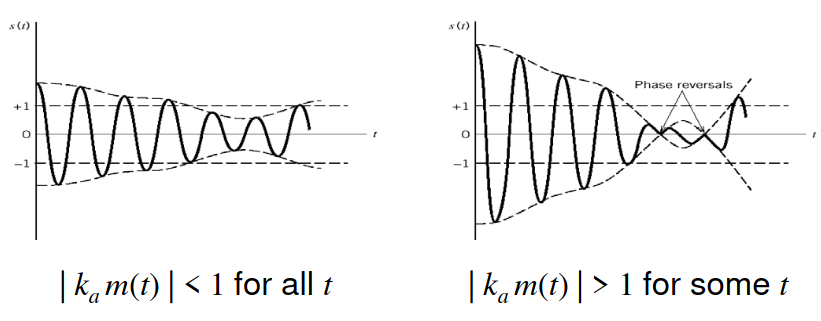
\includegraphics[width = 0.9\linewidth]{img/analog/AM/DSB.png}
    \caption{AM-DSB: onda modulada e sobremodulada, respetivamente.}
    \label{fig:DSB}
\end{figure}

%//==============================--@--==============================//%
\newpage
\subsubsection*{$\rightarrow$ Domínio da frequência}
\label{subsubsec:AM-freq-domain}

Recorrendo à transformada de Fourier, facilmente se obtém o espetro de $s(t)$:

$$
    \boxed{S(f) = \frac{A_c}{2}[\delta(f - f_c) + \delta(f + f_c)] + \frac{k_a A_c}{2}\left[M(f - f_c) + M(f + f_c)\right]}
$$

\noindent onde $M(f)$ é o espetro da mensagem e $M(f)\delta(f - f_c) = M(f - f_c)$, já que $\delta(f)$ é o elemento neutro da convolução.

\begin{figure}[H]
    \centering
    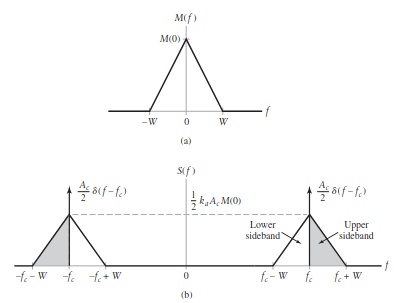
\includegraphics[width = 0.8\linewidth]{img/analog/AM/freqDomain.png}
    \caption{\textbf{(a)} Espetro da mensagem $m(t)$. \textbf{(b)} Espetro da onda modulada $s(t)$.}
    \label{fig:freqDomainDSB}
\end{figure}

\noindent $\pmb{\rightarrow}$ \textbf{\textit{Observações}}
\begin{itemize}
    \item[$\blacktriangle$] ``As a result of the modulation process, the spectrum of the message signal $m(t)$ for negative frequencies extending from $-W$ to 0 becomes completely visible for positive (i.e., measurable) frequencies, provided that the carrier frequency satisfies the condition $f_c >> W$.''\cite{Haykin2007}
    \item[$\blacktriangle$] ``For positive frequencies, the portion of the spectrum of an AM wave lying above the carrier frequency $f_c$ is referred to as the upper sideband, whereas the symmetric portion below $f_c$ is referred to as the lower sideband. The condition $f_c >> W$ ensures that the sidebands do not overlap.''\cite{Haykin2007} (Isto é, o envelope é visualizado).
    \item[$\blacktriangle$]``For positive frequencies, the highest frequency component of the AM wave equals $f_c + W$, and the lowest frequency component equals $f_c - W$. The difference between these two frequencies defines the transmission bandwidth $B_T = 2W$.\cite{Haykin2007}
\end{itemize}

%//==============================--@--==============================//%
\clearpage
\subsubsection[2.1.2 Detetor Envolvente]{$\rightarrow$ Detetor Envolvente}
\label{subsubsec:DetetorEnvolvente}

Admitindo que as \hyperref[subsubsec:AM-freq-domain]{condições supramencionadas} são garantidas, Para recuperar de novo o sinal $m(t)$ partindo da portadora modulada $x_{AM} (t)$ que chega ao recetor, basta rectificar a portadora e filtrar o resultado da rectificação por forma a preservar apenas as flutuações lentas do sinal retificado e que correspondem ao sinal $m(t)$, rejeitando as suas oscilações de alta frequência, usando para o efeito um filtro passa-baixo:

\begin{figure}[H]
    \centering
    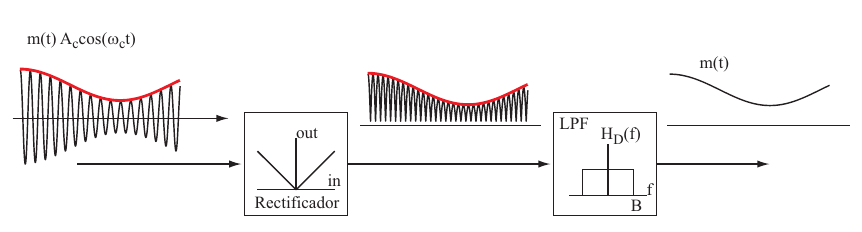
\includegraphics[width = 1\linewidth]{img/analog/AM/detetorEnvolvente.png}
    \caption{Diagrama Detetor Envolvente}
    \label{fig:DetetorEnvolvente}
\end{figure}

\noindent \textbf{$\rightarrow$ Nota}

\noindent A saída do retificador de onda completo é dada por:
$$
    y(t) = s(t) p(t)
$$
Onde $\boxed{p(t) = \text{sgn}[\cos{(2\pi f_c t)}]}$

\begin{figure}[H]
    \centering
    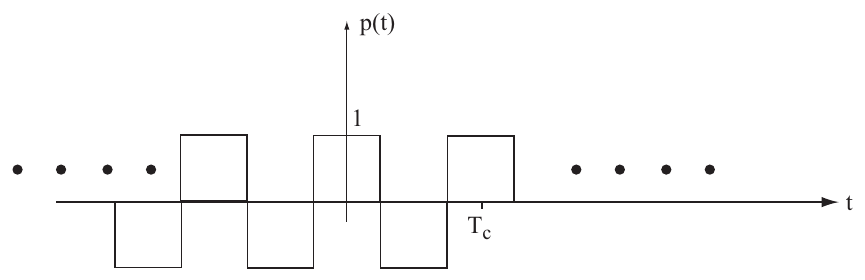
\includegraphics[width = 1\linewidth]{img/analog/AM/pt_envolvente.png}
    \caption{Sinal p(t).}
    \label{fig:p(t)}
\end{figure}

\noindent $p(t)$ é a extensão periódica de $\text{rect}\left(\dfrac{2t}{\text{T}_c}\right)$:

$$
    \boxed{P(f) = \mathcal{F}\{p(t)\} = \sum_{n=-\infty}^{\infty} \text{sinc}(2n)\delta(f - nf_0)}
$$

\noindent Consequentemente $y(t)$ possui uma réplica centrada em $f = 0$ que pode ser usada para recuperar integralmente o sinal $m(t)$ após filtragem pelo filtro de saída do detetor de envolvente.
\\\\
\noindent Por fim admite-se que à sa\'ida do receptor existe um condensador com a finalidade de remover a componente DC, $m_{dc}$ advinda do envelope, $[m_{dc} + k_a m(t)]$.

%//==============================--@--==============================//%
\subsubsection[2.1.3 Double Sideband Supressed Carrier]{$\rightarrow$ Double Sideband Supressed Carrier}
\label{subsubsec:DSB-SC}

``Basically, double sideband-suppressed carrier (DSB-SC) modulation consists of the product of the message signal $m(t)$ and the carrier wave $c(t)$, as shown in the equation:''\cite{Haykin2007}

$$
    \boxed{s(t) = c(t) m(t) = m(t) A_c \cos{(2\pi f_c t)}}
$$

\noindent Contrariamente à modulação anteriormente discutida, a modulação DSB-SC é anulada com o desaparecimento da mensagem de modulação. Neste sentido ``Transmitted power is saved here through the suppression of the carrier wave''\cite{Haykin2007} embora a largura de banda do canal se mantenha idêntica, nomeadamente $B_t = 2W$.
%//==============================--@--==============================//%
\subsubsection*{$\rightarrow$ Domínio da frequência}
\label{subsubsec:AM-freq-domain DSB-SC}

A transformada de Fourier de $s(t)$ é dada por

$$
    \boxed{S(f) = \frac{A_c}{2}\left[M(f - f_c) + M(f + f_c)\right]}
$$

\begin{figure}[H]
    \centering
    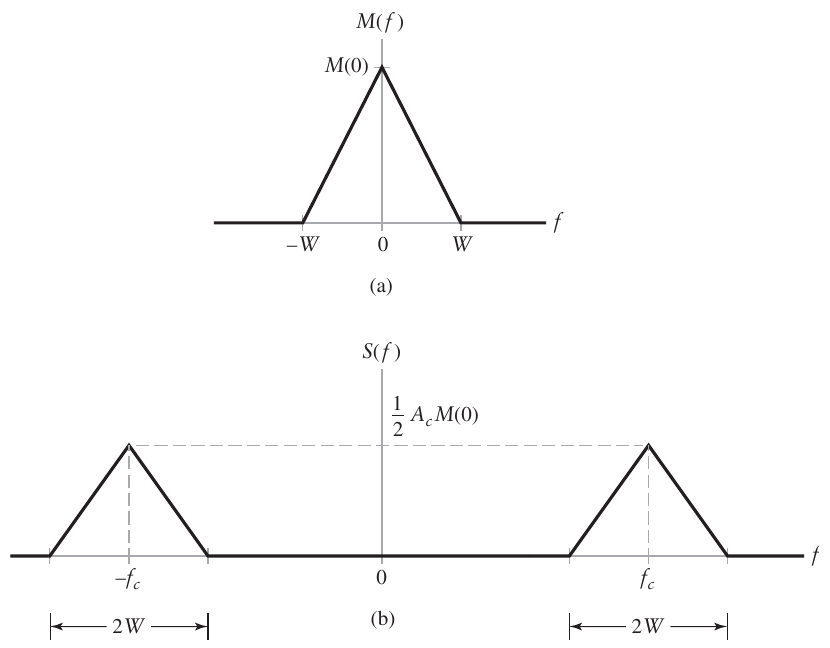
\includegraphics[width = 0.8\linewidth]{img/analog/AM/freqDomainDSB-DC.png}
    \caption{\textbf{(a)} Espetro da mensagem $m(t)$. \textbf{(b)} Espetro da onda modulada $s(t)$.}
    \label{fig:FreqDSB-DC}
\end{figure}

\noindent $\pmb{\rightarrow}$ \textbf{\textit{Observações}}
\begin{itemize}
    \item[$\blacktriangle$] ``Except for a change in scale factor, the modulation process simply translates the spectrum of the message signal by $f_c$ to the right and by $-f_c$ to the left. Of course, the transmission bandwidth required by DSB-SC modulation is the same as that for amplitude modulation namely, 2W.''\cite{Haykin2007}
\end{itemize}


%//==============================--@--==============================//%
\clearpage
\subsubsection[2.1.4 Detetor Coerente]{$\rightarrow$ Detetor Coerente}
\label{subsubsec:DetetorCoerente}
Se a amplitude do sinal modulante mudar de um valor positivo para um valor negativo, irá provocar inversões de fase na portadora modulada. Tal fenómeno é visível em casos de sobremodulação, inerentes à modulação DSB-SC, à qual o detetor envolvente é insensível. É então usado um desmodulador imune às inversões de fase, denominado detetor coerente ou síncrono:

\begin{figure}[H]
    \centering
    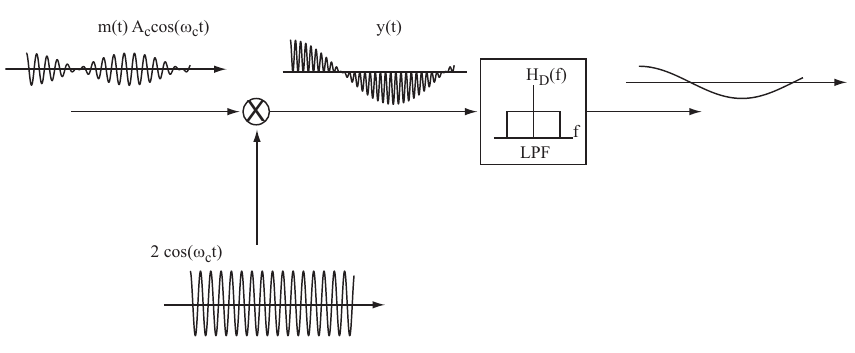
\includegraphics[width = 1\linewidth]{img/analog/AM/detetorSincrono.png}
    \caption{Diagrama do detetor coerente.}
    \label{fig:detetorCoerente}
\end{figure}

\noindent Avaliando o sinal à saída do modulador de produto (``assuming that the
local oscillator is out of phase by $f$ with respect to the sinusoidal carrier
 oscillator in the transmitter.''\cite{Haykin2007})

 $$
    y(t) = A'_c\cos{(2\pi f_c t + \Phi)}
 $$

%//==============================--@--==============================//%
\subsubsection[2.1.5 Potência de transmissão de uma onda modulada em amplitude]{$\rightarrow$ Potência de transmissão de uma onda modulada em amplitude}
\label{subsubsec:AM-power}

Tomando uma onda AM arbitrária da forma:
$$
    x_{\text{AM}}(t) = A_c[m_{dc} + m(t)] \cos(2\pi f_c t) 
$$
Verifica-se que a potência média do sinal, i.e., $<x_{\text{AM}}(t)>$ é dada por
$$
    P_T = \frac{A^2_c}{2}\left( m_{dc}^2 + P_m \right)
$$
em que $P_m$ é a potência média do sinal mensagem.

\paragraph[2.1.5.1 Eficiência de modulação de um sinal AM]{$\pmb{\star}$ Eficiência de modulação de um sinal AM}\mbox{}\\
 ``We define modulation efficiency as the ratio between the power of the part of the modulated signal that carries information about $m(t)$ and the total power of the modulated signal.''\cite{Nunes2015}
 $$
    \eta \delequal \frac{(A^2_c/2)P_m}{P_T} = \frac{P_m}{P_m + m_{dc}^2}
 $$
%//==============================--@--==============================//%